% !TEX root = tesis.tex

\chapter{Telescopio centellador de Rayos Cósmicos}
\chaptermark{Telescopio centellador}
\label{chap:dos}

Actualmente los telescopios de neutrones solares solo permiten estudiar el espectro de energía de manera parcial, es decir, con resolución limitada. Dado que los neutrones tienen masa, sus velocidades sufren dispersión dependiendo de su energía, lo cual complica establecer el perfil temporal de emisión. Aunado a esto, la baja estadística de conteo producto de la eficiencia de los telescopios y su limitada resolución angular; limitan las posibilidades de los TNS para esclarecer los mecanismos de aceleración de partículas.

Un diseño mejorado de Telescopio de neutrones fue propuesto en \cite{sako03}. En este diseño se utilizan barras de centelleo de dimensiones \SI[product-units=power]{5x10x300}{\cm}, alineadas de tal forma que permiten trazar las trayectorias de los neutrones incidentes además de medir su energía depositada. El Telescopio centellador de Rayos cósmicos (\emph{SciCRT} por sus siglas en inglés) es un nuevo experimento de rayos cósmicos basado en este principio.

El SciCRT utiliza como trazador activo el detector \emph{SciBar}, diseñado originalmente para el experimento \emph{long-baseline K2K} \cite{knitta04} y posteriormente en el experimento \emph{SciBooNE} del \emph{Fermilab} (Laboratorio Nacional Fermi) \cite{hiraide06}. En el año \num{2013} el SciBar fue trasladado a la cima del volcán Sierra Negra, Puebla a \SI{4600}{\metre} sobre el nivel del mar, con el objetivo de observar neutrones solares. La localidad de Sierra Negra es ideal para este experimento debido a la profundidad atmosférica (en línea vertical: \SI{575}{\gram\per\square\centi\metre}), su cercanía con el ecuador terrestre ($\ang{19.0}\mathbf{N}$, $\ang{97.3}\mathbf{W}$) , además de la experiencia previa en la operación de otro telescopio de neutrones solares en el sitio y la infraestructura del lugar\footnote{En la actualidad el volcán Sierra Negra se ha convertido en un observatorio astrofísico de nivel mundial.}.

Un diagrama esquemático del detector se muestra en la figura \ref{fig:scibar-detector}. Las ventajas del SciCRT sobre la generación previa de telescopios proviene de integrar las funciones de anti-coincidencia, blanco centellador y telescopio direccional en las barras centelleo del SciBar. Esto permite tener \num{15} veces más volumen activo, mejor resolución en energía y un umbral de detección menor. Considerando todas estas características el SciCRT tiene una eficiencia detección \num{10} veces mayor a la del TNS previamente en el mismo sitio \cite{ynagai14} (considerando neutrones de \SI{100}{\mega\electronvolt}).

\begin{figure}
        \centering
        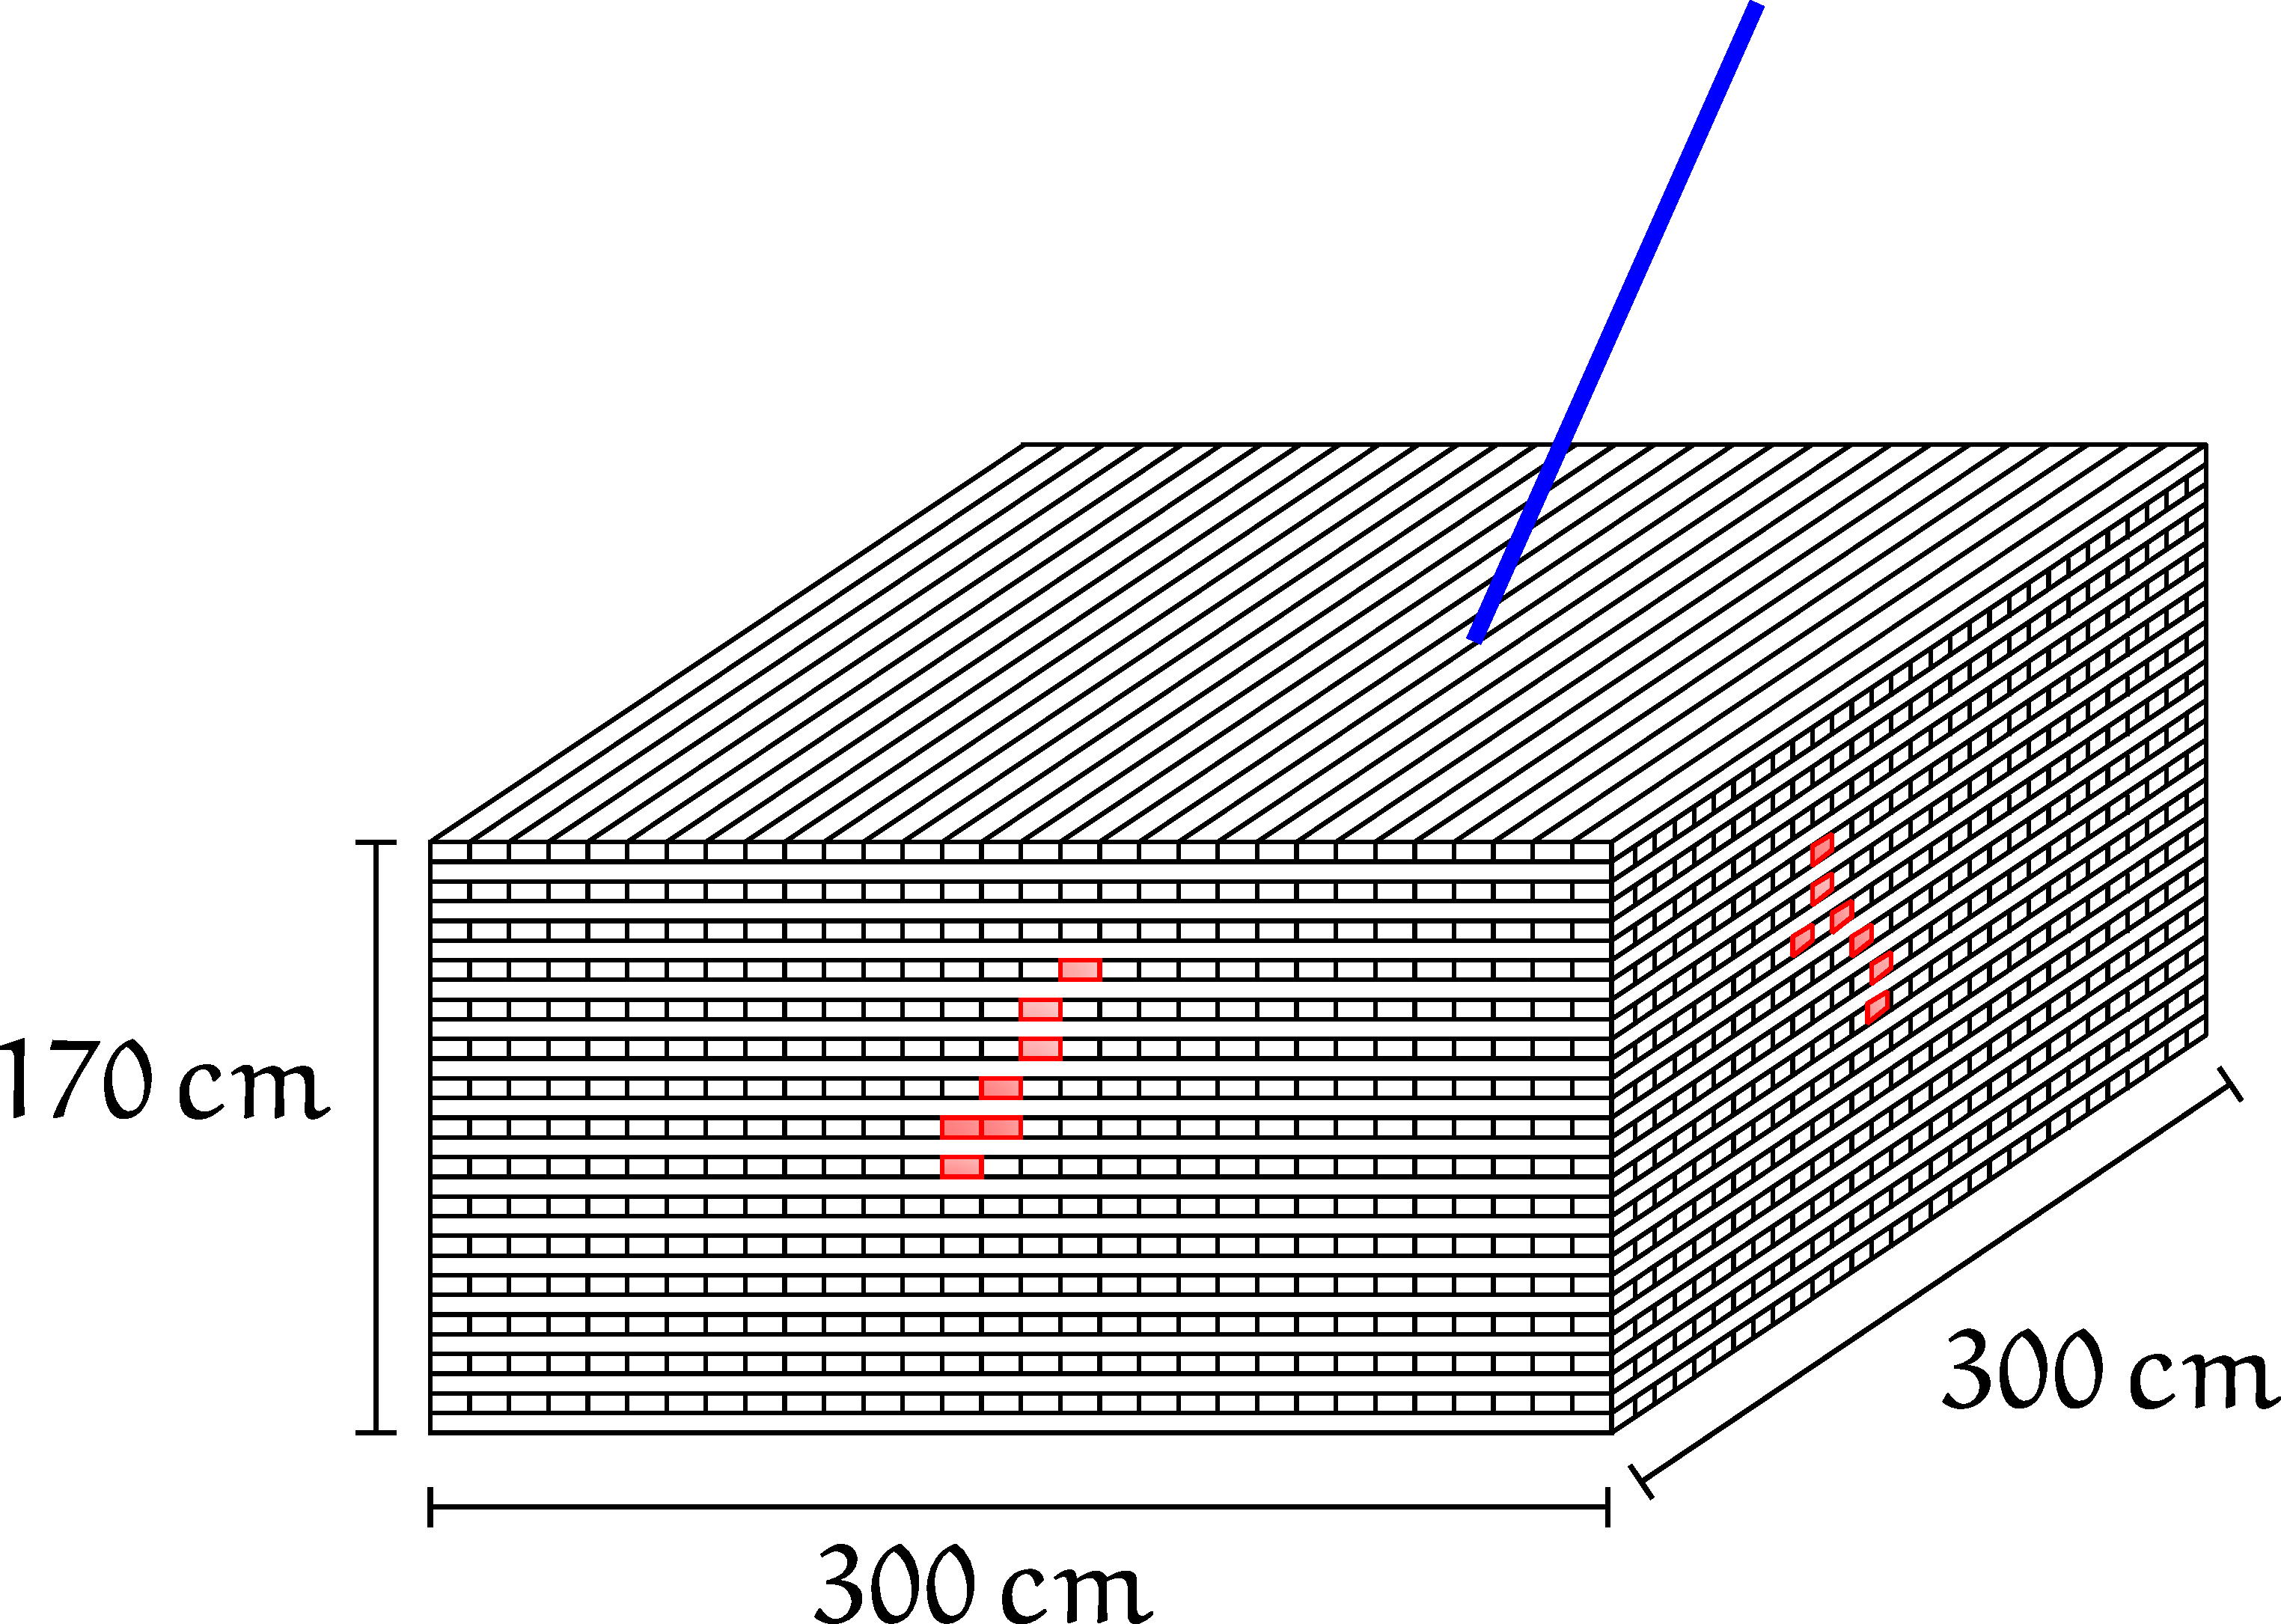
\includegraphics[width=0.7\textwidth]{scibar-diagram.pdf}
        \caption{Diagram esquemático del SciCRT. El detector se compone de \num{14848} barras centelladoras y fibras WLS. La lectura de las fibras se hace por medio MAPMTs en grupos de \num{64} canales.}
        \label{fig:scibar-detector}
\end{figure}

Por otro lado, dado que el SciCRT registra la energía depositada a lo largo la trayectoria de las partículas dentro del detector, podemos aplicar esquemas novedosos de identificación de partículas; lo cual a su vez mejora la sensibilidad a las partículas solares \cite{garcia20}. Este tipo de análisis \emph{offline} en conjunción con el uso de las barras de centelleo en modo anti-coincidencia mejora el rechazo a partículas de fondo (principalmente $\mu^{\pm}$ y rayos $\gamma$) incrementando la razón señal a ruido.

\section{Descripción del detector}

El SciCRT está compuesto de \num{14848} barras de centelleo, alineadas en planos horizontales $X-Y$, perpendiculares entre si. Los planos están constituidos de \num{116} barras en la dirección $X$ y \num{118} en la dirección $Y$. En total hay \num{128} capas de barras de centelleo apiladas verticalmente, agrupada en estructuras de \num{16} capas llamadas \emph{Super block} (SB). Cada SB está sostenido firmemente por una estructura de acero, la cual mantiene la integridad mecánica de las barras. No obstante, la estructura introduce un hueco de aire entra cada capa de \SI{82}{\mm}, lo cual entre otras cosas afecta la respuesta angular del telescopio; por lo que es necesario incluir esta característica en las simulaciones del detector. El volumen total del barras en el detector es de \SI[product-units=power]{300x300x170}{\cm\cubic}.

Las barras de centelleo fueron fabricadas en el Fermilab y tienen características similares a las del experimento \emph{MINOS} \cite{knitta04}. Están hechas de poliestireno, dopado con \SI{1}{\percent} PPO and \SI{0.03}{\percent} POPOP (ambos utilizados como \emph{cambiadores} de longitud de onda). Las dimensiones de las barras son \SI[product-units=power]{2.5x1.3x300}{\cm\cubic} y en el centro tienen un orificio cilíndrico de \SI{1.8}{\mm} donde se insertan fibras WLS (\emph{wavelength shifting}). Los centelladores tienen una cubierta de \ce{TiO2} (\SI{0.25}{\mm} de espesor) para aislarlos ópticamente entre si y mejorar la recolección de fotones. Un diagrama de las barras se observa en el panel izquierdo de la figura \ref{fig:scibar-optics}.

Las fibras WLS están acopladas por un lado a un tubo fotomultiplicador multi-ánodo (MAPMT) y por el otro extremo están pintadas de blanco para mejorar la eficiencia de recolección. Las fibras son del tipo Y11(200)MS desarrollado por la empresa \emph{Kuraray}. El fotomultiplicador es de \num{64} canales, modelo H8804, fabricado por \emph{Hamamatsu Photonics}.

El espectro de emisión de los plásticos centelladores se puede observar en el panel derecha de la figura \ref{fig:scibar-optics}, con una respuesta máxima a \SI{420}{\nano\metre}. Como se observa en la figura, el espectro de absorción de la fibra WLS está diseñado para cubrir de forma adecuada el espectro del plástico. La emisión de la fibra tiene un máximo a \SI{470}{\nano\metre}. La máxima eficiencia cuántica del MAPMT es de \num{0.25} a \SI{420}{\nano\metre}, pero disminuye a \num{0.12} al considerar el respuesta espectral del MAPMT.

\begin{figure}
        \centering
        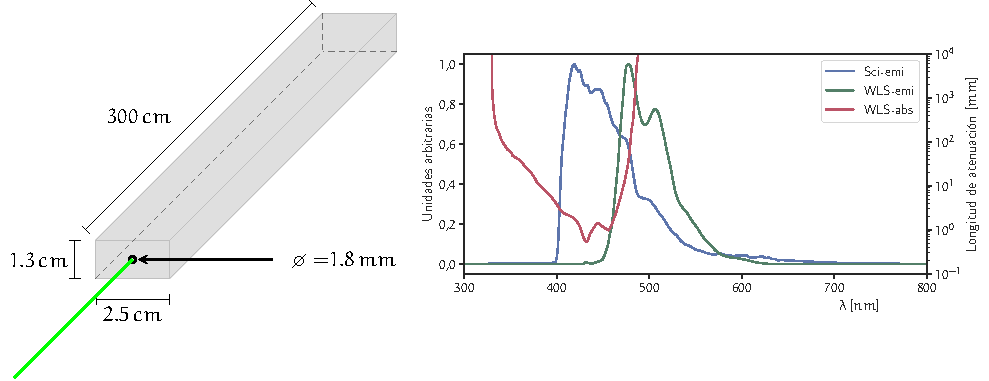
\includegraphics[width=\textwidth]{scibar.pdf}
        \caption{Diagrama esquemático de una barra centelladora con la fibra WLS instalada (panel izquierdo). Espectros de absorción y emisión de la fibra WLS y la barra de centelleo. Los datos de los espectros fueron obtenidos de \cite{kikawa14} y \cite{dietz16}.}
        \label{fig:scibar-optics}
\end{figure}

La electrónica para la adquisición de datos del telescopio fue desarrollada para el experimento K2K y esta integrada por circuitos de procesamiento analógico, de señal mixta y digitales; integrados a través de tecnología de circuitos integrados de alta escala \cite{myoshi04}. El procesamiento de la señales empieza con la conversión de la señal óptica en eléctrica por parte del MAPMT, para posteriormente ser amplificada, formada y multiplexada en la electrónica de \emph{Front End}. Este acondicionamiento se lleva a cabo en el dominio analógico y de señal mixta. Después de este proceso, las señales se transfieren a la electrónica de \emph{Back End} mediante un bus diferencial. En las unidades que integran la electrónica de BE las señales son convertidas a digital y transferidas finalmente al servidor de adquisición de datos mediante la interface VME. Para poder seleccionar los eventos a guardar, las unidades FE mandan una señal de \emph{hit} a las tarjetas de disparo (TRGB), las cuales son unidades de procesamiento digital programable, que seleccionan los eventos con base a una condición de disparo. Una discusión más profunda sobre el funcionamiento de la electrónica se encuentra en el capitulo \ref{chap:tres}, en donde además se listan requerimientos y características de la nueva electrónica a desarrollar.

Bajo condiciones normales, el telescopio registra dos conjuntos de datos diferentes. Muones de alta energía (arriba de \SI{450}{\mega\electronvolt}) son detectados cuando producen coincidencia en las capas superiores e inferiores del detector. El umbral para la detección de partículas en las capas dedicadas es de \SI{0.3}{MIP} (\SI{\approx 0.5}{\mega\electronvolt}). El otro conjunto de datos del telescopio registra partículas neutras (aproximadamente \SI{70}{\percent} de los datos son de neutrones atmosféricos). El disparo para este tipo de eventos está definido cuando no hay ninguna señal en la capa de muones (anti-coincidencia) y además se registra una traza en uno de los SB con al menos \SI{14}{\mega\electronvolt} de energía depositada. Las ganancias de los MAPMT y umbrales para las capas de neutrones y muones se determinaron mediante simulaciones MC y se calibraron en Abril de \num{2014} \cite{ysasai14}.

\subsection{Sistema opto-electrónico}

Para lograr alcanzar los objetivos planteados, la caracterización de los elementos ópticos y opto-electrónicos que integran al SciCRT es de vital importancia.

Como ya se mencionó, las barras de centelleo del detector fueron fabricadas por Fermilab y sus propiedades ópticas (y mecánicas) fueron probadas



\begin{figure}
        \centering
        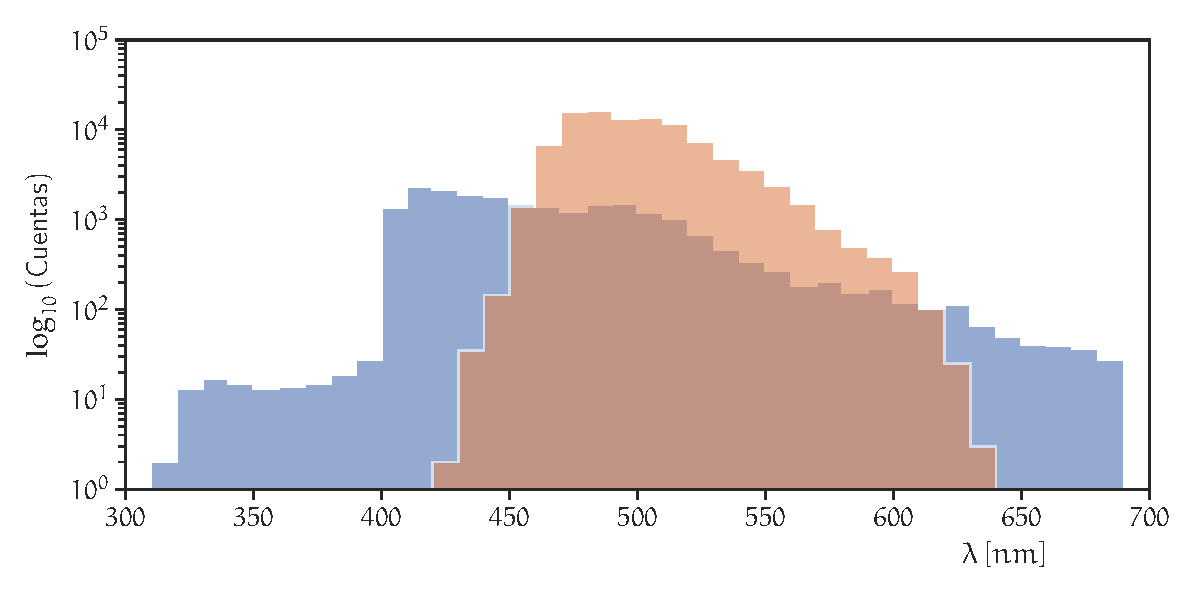
\includegraphics[width=\textwidth]{sim-optics-spect.pdf}
        \caption{Simulación MC del proceso de emisión-absorción de fotones entre la barra y la fibra WLS.}
        \label{fig:sim-optics}
\end{figure}

\begin{equation}
\label{equ:fiber-att}
L(x)=k\left(\exp\left(-\frac{x}{\lambda}\right) +R\exp\left(-\frac{2.0x_{tot}-x}{\lambda}\right)\right)
\end{equation}

\begin{figure}
        \centering
        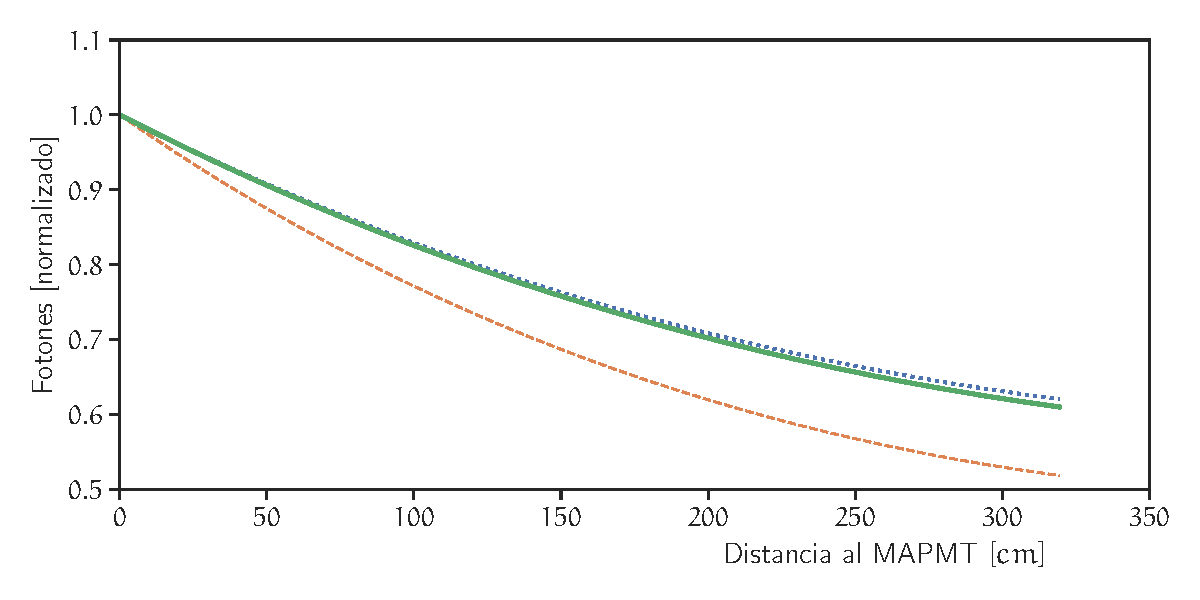
\includegraphics[width=\textwidth]{data_atlength.pdf}
        \caption{Atenuación de fotones en la fibra WLS. La línea azul son datos del experimento. La línea naranja representa el resultado de la simulación MC usando la atenuación reportada por el fabricante. La línea verde es el ajuste de la simulación a partir del experimento.}
        \label{fig:atlength}
\end{figure}

\begin{figure}
        \centering
        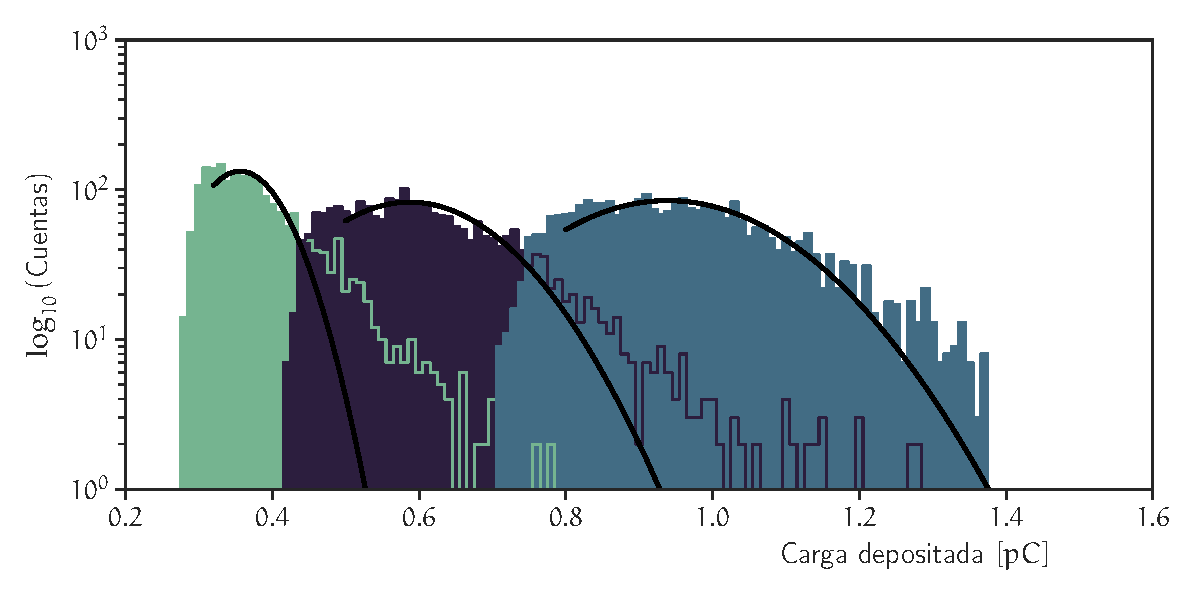
\includegraphics[width=\textwidth]{mapmt_charge.pdf}
        \caption{Distribuciones de carga de SPE para tres diferentes voltajes de operación. De izquierda a derecha los voltajes utilizados son: \SI{-800}{\volt},\SI{-850}{\volt} y \SI{-900}{\volt}.}
        \label{fig:mapmt_charge}
\end{figure}

\begin{equation}
\label{equ:sphe}
v(t)=\frac{QR}{\tau\Gamma(1+\alpha)}\left(\frac{t}{\tau}\right)^{\alpha}\mathrm{e}^{-t/\tau}
\end{equation}

\begin{figure}
        \centering
        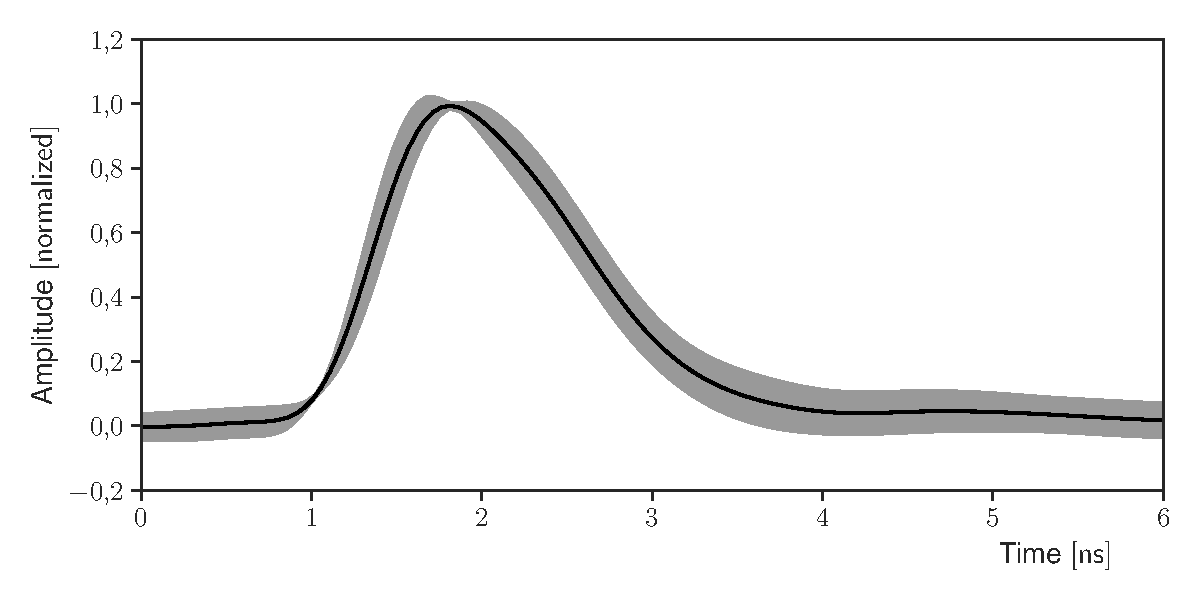
\includegraphics[width=\textwidth]{sphe-signal.pdf}
        \caption{Respuesta SPE promedio en función del tiempo (linea negra). El área sombreada muestra las fluctuaciones de $\pm\sigma$.}
        \label{fig:sphe}
\end{figure}

\begin{figure}
        \centering
        \includegraphics[width=\textwidth]{muons-experiment.pdf}
        \caption{Configuración del experimento en Sierra Negra. El sistema de coincidencias se forma por las tarjetas instaladas en las posiciones marcadas en verde.}
        \label{fig:muons-experiment}
\end{figure}


\begin{figure}
        \centering
        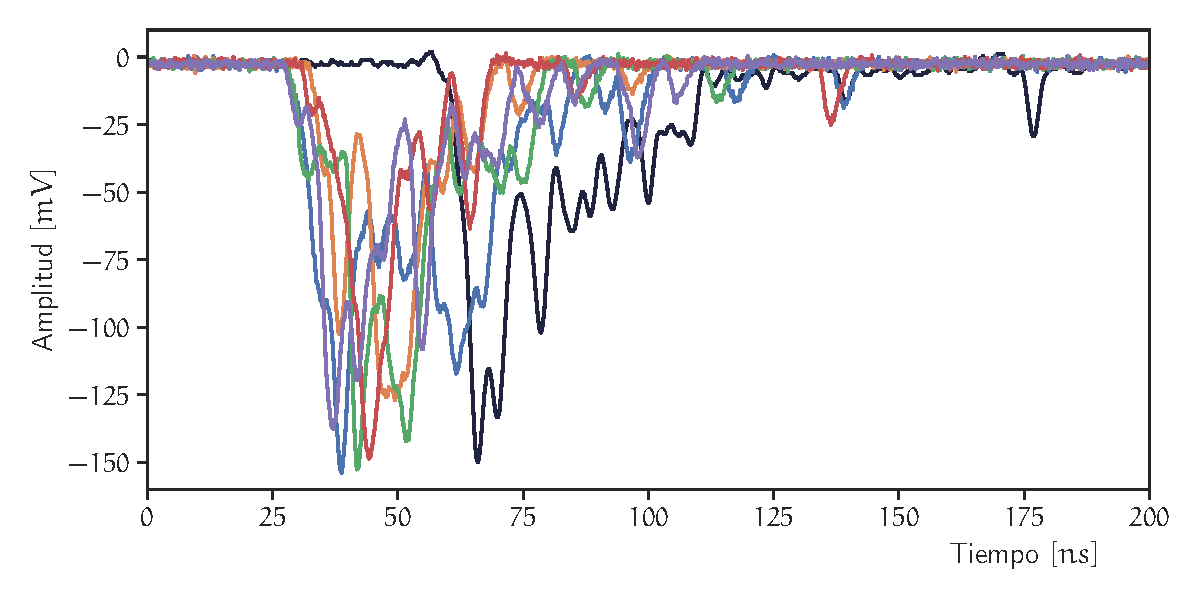
\includegraphics[width=\textwidth]{muon-pulse.pdf}
        \caption{Comparación entre señales generadas por la simulación MC (líneas de color) y el experimento realizado en Sierra Negra (línea oscura).}
        \label{fig:muon-pulse}
\end{figure}

\begin{figure}
        \centering
        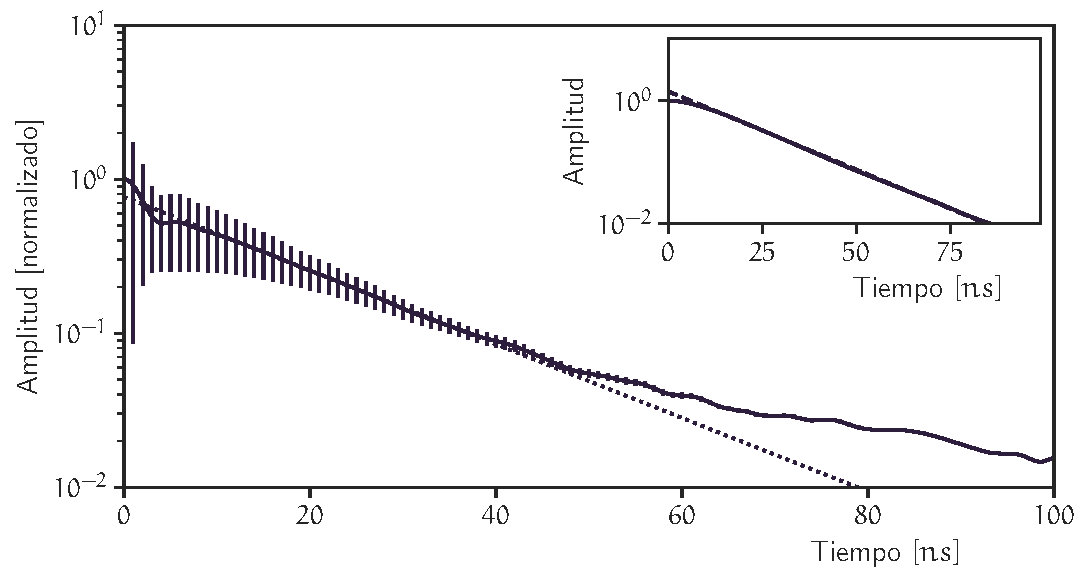
\includegraphics[width=\textwidth]{muons-tail-fit.pdf}
        \caption{Análisis del decaimiento exponencial de la fibra WLS. El panel en la esquina superior derecha muestra los resultados de la simulación. Los datos experimentales se muestran en la parte central de la figura}
        \label{fig:muons-tail}
\end{figure}

\begin{equation}
\label{equ:nphe}
s(N_{phe})=\frac{1}{k_{sat}}\int_{0}^{N_{max}} s_{sim}(N_{sim})p(N_{phe}-N_{sim})\;\mathrm{d}N_{sim}
\end{equation}

\begin{figure}
        \centering
        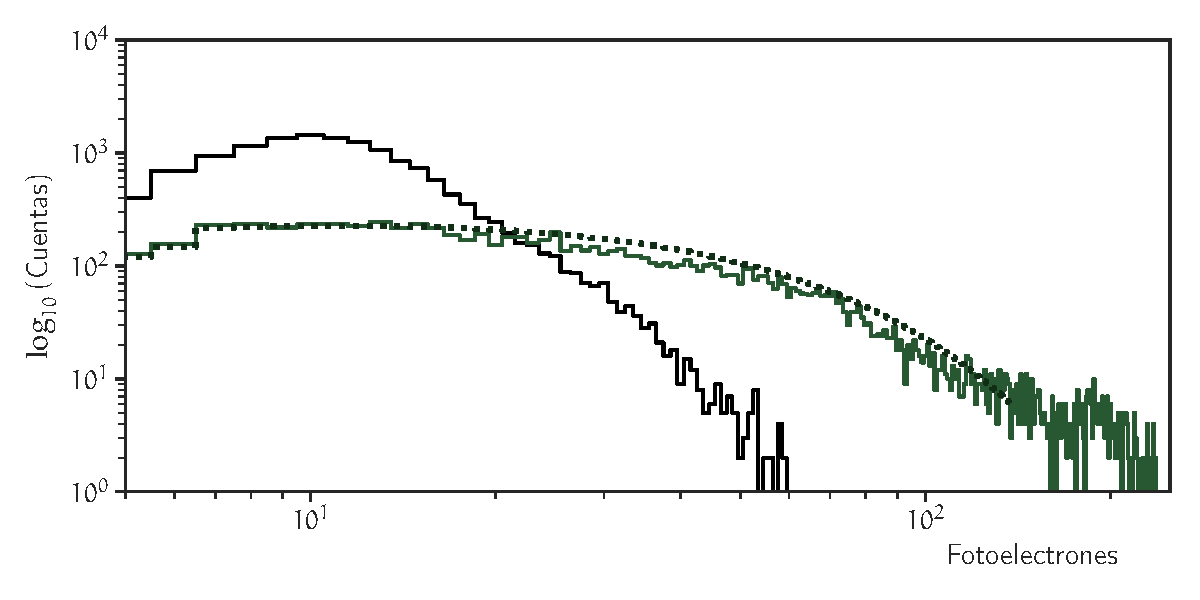
\includegraphics[width=\textwidth]{photons-number.pdf}
        \caption{Distribución de número de fotoelectrones detectados en el experimento y la simulación MC. Los resultados de la simulación se convolucionan con una función de resolución para ajustar con los datos experimentales.}
        \label{fig:photons-number}
\end{figure}
